%++++++++++++++++++++++++++++++++++++++++
\documentclass[article, 12pt]{article}
\usepackage{float}
\usepackage{setspace}
\usepackage{tabu} % extra features for tabular environment
\usepackage{amsmath}  % improve math presentation
\usepackage{graphicx} % takes care of graphic including machinery
\usepackage[margin=1in]{geometry} % decreases margins
\usepackage{cite} % takes care of citations
\usepackage[final]{hyperref} % adds hyper links inside the generated pdf file
\usepackage{tikz}
\usepackage{caption} 
\usepackage{fancyhdr}
\usepackage{amssymb} % symbols like /therefore
\usepackage{amsthm} % proofs
\usepackage{enumerate} % lettered lists
\usepackage{mathtools} % macros
\usepackage{multirow} % multirow tables
\usetikzlibrary{scopes}
% \usepackage{xcolor} \pagecolor[rgb]{0.12549019607,0.1294117647,0.13725490196} \color[rgb]{0.82352941176,0.76862745098,0.62745098039} % dark theme
\hypersetup{
	colorlinks=true,       % false: boxed links; true: colored links
	linkcolor=blue,        % color of internal links
	citecolor=blue,        % color of links to bibliography
	filecolor=magenta,     % color of file links
	urlcolor=blue         
}
\usepackage{physics}
\usepackage{siunitx}
\usepackage{tikz,pgfplots}
\usepackage[outline]{contour} % glow around text
\usetikzlibrary{calc}
\usetikzlibrary{angles,quotes} % for pic
\usetikzlibrary{arrows.meta}
\tikzset{>=latex} % for LaTeX arrow head
\contourlength{1.2pt}

\colorlet{xcol}{blue!70!black}
\colorlet{vcol}{green!60!black}
\colorlet{myred}{red!70!black}
\colorlet{myblue}{blue!70!black}
\colorlet{mygreen}{green!70!black}
\colorlet{mydarkred}{myred!70!black}
\colorlet{mydarkblue}{myblue!60!black}
\colorlet{mydarkgreen}{mygreen!60!black}
\colorlet{acol}{red!50!blue!80!black!80}
\tikzstyle{CM}=[red!40!black,fill=red!80!black!80]
\tikzstyle{xline}=[xcol,thick,smooth]
\tikzstyle{mass}=[line width=0.6,red!30!black,fill=red!40!black!10,rounded corners=1,
                  top color=red!40!black!20,bottom color=red!40!black!10,shading angle=20]
\tikzstyle{faded mass}=[dashed,line width=0.1,red!30!black!40,fill=red!40!black!10,rounded corners=1,
                        top color=red!40!black!10,bottom color=red!40!black!10,shading angle=20]
\tikzstyle{rope}=[brown!70!black,very thick,line cap=round]
\def\rope#1{ \draw[black,line width=1.4] #1; \draw[rope,line width=1.1] #1; }
\tikzstyle{force}=[->,myred,very thick,line cap=round]
\tikzstyle{velocity}=[->,vcol,very thick,line cap=round]
\tikzstyle{Fproj}=[force,myred!40]
\tikzstyle{myarr}=[-{Latex[length=3,width=2]},thin]
\def\tick#1#2{\draw[thick] (#1)++(#2:0.12) --++ (#2-180:0.24)}
\DeclareMathOperator{\sn}{sn}
\DeclareMathOperator{\cn}{cn}
\DeclareMathOperator{\dn}{dn}
\def\N{80} % number of samples in plots


\usepackage{titling}
\renewcommand\maketitlehooka{\null\mbox{}\vfill}
\renewcommand\maketitlehookd{\vfill\null}
\usepackage{siunitx} % units
\usepackage{verbatim} 
\newcommand{\labTitle}{Solid Pendulum}
\newcommand{\class}{AP Physics C}
\newcommand{\professor}{Mr. Perkins}
\newcommand{\name}{Denny Cao}
\pagestyle{fancy}
\fancyhf{}% clears all header and footer fields
\fancyfoot[C]{--~\thepage~--}
\renewcommand*{\headrulewidth}{0.4pt}
\renewcommand*{\footrulewidth}{0pt}
\lhead{\name}
\chead{\class: \labTitle}
\rhead{\professor}


\fancypagestyle{plain}{%
  \fancyhf{}% clears all header and footer fields
  \fancyfoot[C]{--~\thepage~--}%
  \renewcommand*{\headrulewidth}{0pt}%
  \renewcommand*{\footrulewidth}{0pt}%
}

% Shortcuts
\DeclarePairedDelimiter\ceil{\lceil}{\rceil} % ceil function
\DeclarePairedDelimiter\floor{\lfloor}{\rfloor} % floor function

\DeclarePairedDelimiter\paren{(}{)} % parenthesis

\newcommand{\df}{\displaystyle\frac} % displaystyle fraction
\newcommand{\qeq}{\overset{?}{=}} % questionable equality

\newcommand{\Mod}[1]{\;\mathrm{mod}\; #1} % modulo operator

% Sets
\DeclarePairedDelimiter\set{\{}{\}}
\newcommand{\unite}{\cup}
\newcommand{\inter}{\cap}

\newcommand{\reals}{\mathbb{R}} % real numbers: textbook is Z^+ and 0
\newcommand{\ints}{\mathbb{Z}}
\newcommand{\nats}{\mathbb{N}}
\newcommand{\rats}{\mathbb{Q}}

\newcommand{\degree}{^\circ}
\newcommand{\tplint}[6]{\int\limits^{#1}_{#2}\int\limits^{#3}_{#4}\int\limits^{#5}_{#6}} % triple integral bounds
% Counting
\newcommand{\dblint}[4]{\int\limits^{#1}_{#2}\int\limits^{#3}_{#4}} % double integral bounds
\newcommand{\sglint}[2]{\int\limits^{#1}_{#2}} % integral bounds
\newcommand\perm[2][^n]{\prescript{#1\mkern-2.5mu}{}P_{#2}}
\newcommand\comb[2][^n]{\prescript{#1\mkern-0.5mu}{}C_{#2}}

\setlength\parindent{0pt}

% Sign Charts
\newdimen\tcolw \tcolw=2.5em % the column width
\edef\ecatcode{\catcode`&=\the\catcode`&\relax}\catcode`&=4
\def\sgchart#1#2{\vbox{\offinterlineskip\halign{\hfil##\quad&##\hfil\crcr\sgchartA#2,:,%
   \omit\sgchartR&\kern.2pt\sgchartS{.5\tcolw}\relax\sgchartE#1,\relax,%
   \sgchartS{.5\tcolw}\relax\cr
   \noalign{\kern2pt}&\def~{}\kern.5\tcolw\sgchartD#1,\relax,\cr}}}
\def\sgchartA#1:#2,{\cr\ifx,#1,\else $#1$&\sgchartB#2{}\expandafter\sgchartA\fi}
\def\sgchartB#1{\hbox to\tcolw{\hss$#1$\hss}\sgchartC}
\def\sgchartC#1{\ifx,#1,\else
   \strut\vrule\kern-.4pt\hbox to\tcolw{\hss$#1$\hss}\expandafter\sgchartC\fi}
\def\sgchartD#1#2,{\ifx\relax#1\else\hbox to\tcolw{\hss$#1#2$\hss}\expandafter\sgchartD\fi}
\def\sgchartE#1#2,{\ifx\relax#1\else
    \ifx~#1\sgchartS\tcolw\circ \else\sgchartS\tcolw\bullet\fi \expandafter\sgchartE\fi}
\def\sgchartR{\leaders\vrule height2.8pt depth-2.4pt\hfil}
\def\sgchartS#1#2{\hbox to#1{\kern-.2pt\sgchartR \ifx\relax#2\else
   \kern-.7pt$#2$\kern-.7pt\sgchartR\fi\kern-.2pt}}
\ecatcode
%++++++++++++++++++++++++++++++++++++++++
\title{
    \vspace{2in}
    \textmd{\textbf{\labTitle}}
    \normalsize\vspace{0.1in}\\
    \vspace{0.1in}\large{\text{\class: \professor}}
    \vspace{3in}
}

\author{\name}
\date{December 21, 2022}

\begin{document}
    \maketitle
    \thispagestyle{empty}
    \pagebreak
    \section*{Introduction}
    The goal of this lab is to be able to use concepts of torque, simple harmonic motion (SMH), and moment of inertia to completely describe the motion of a solid body that pivots at some arbitrary point.
    \section{Case 1: The Pendulum Bob (Concentrated Mass)}
    \subsection{Procedure}
    We determined the variables that affect the period of a pendulum bob by suspending a 100 gram mass from a string. We tested two variables: angle and radius (length of the string). With each trial, we timed 10 oscillations to determine the period.
    \subsection{Data}
    \begin{table}[H]
        \centering
        \begin{tabular}{|c|c|c|}
            \hline
            \textbf{Angle (\SI{}{\degree})} & \textbf{Time of 10 Swings (\SI{}{\second})} & \textbf{Period} ($\text{s}/\text{cycle}$ \\
            \hline
            5  & 15.32 & 1.532 \\
            30 & 15.49 & 1.549 \\
            45 & 15.77 & 1.577 \\
            \hline
        \end{tabular}
        \caption{Period of \SI{0.63}{\meter} String at Various Angles}
        \label{tab:angle}
    \end{table}
    From \autoref{tab:angle}, since there is a relatively small difference in period, we can conclude that the period of a pendulum bob is negligibly impacted by the angle of the string from the vertical---the amplitude. \\
    \\
    We then tested the effect of the length of the string on the period of the pendulum bob. From our previously conclusion, we can assume that the period is independent of the angle of the string from the vertical. \\
    \begin{table}[H]
        \centering
        \begin{tabular}{|c|c|c|}
            \hline
            \textbf{Length of String} (\SI{}{\meter}) & \textbf{Time of 10 Swings} (\SI{}{\second}) & \textbf{Period} ($\text{s}/\text{cycle}$) \\
            \hline
            0.63 & 15.63 & 1.563 \\
            0.48 & 14.05 & 1.405 \\
            0.30 & 10.97 & 1.097 \\
            0.18 & 8.29  & 0.829 \\
            0.05 & 4.42  & 0.442 \\ 
            \hline
        \end{tabular}
        \caption{Observed Period of Pendulum for Different Lengths of String}
        \label{tab:observedPeriod}
    \end{table}
    \subsection{Analysis}
    \begin{enumerate}[1)]
        \item \textbf{Does the amplitude influence the period?  Does a 1 degree amplitude give a smaller period than a 10 degree amplitude?  What if the angle is greater than 15 degrees?}

        By changing the angle, we thereby change the amplitude. From \autoref{tab:angle}, the mean period for a string of length 0.63 meters is:
        \begin{equation}            \label{eq:mean}
            \mu = \frac{1.532 + 1.549 + 1.577}{3} \approx 1.5527 \text{ seconds}
        \end{equation}
    We then calculate the standard deviation of the period:
    \begin{equation}        \label{eq:std}
        \sigma = \sqrt{\frac{1}{3}\sum_{i=1}^{3}(x_i - \mu)^2} \approx 0.0186 \text{ seconds}
    \end{equation}
    Since the standard deviation is less than 0.02 seconds, we can conclude that the period of a pendulum bob is independent of the amplitude of the pendulum bob. The variance is most likely attributed to the fact that we manually timed the period of the pendulum bob. \\
    \item \textbf{Draw an FBD for the pendulum at some point in the swing.  Show the restoring force.}
    \begin{figure}[H]
        \centering
    % PENDULUM
    \def\L{4}  % string length
    \def\ang{30} % angle string
    \def\R{0.25} % ball radius
    \def\F{1.0}  % force magnitude
    \begin{tikzpicture}
    \coordinate (M) at (\ang-90:\L);
    \coordinate (M') at (0,-\L);
    \coordinate (O) at (0,0);
    \coordinate (B) at (0,-\L-2.2*\R);
    \coordinate (FT) at ($(M)+(90+\ang:{\F*cos(\ang)+\R})$);
    \coordinate (FG) at ($(M)+(-90:{\F+\R})$);
    \coordinate (FGx) at ($(M)+(-90+\ang:{0.55*\F+\R})$);
    \coordinate (MA) at ($(M)+(180+\ang:{\F*sin(\ang)+\R})$);
    %\draw[faded mass] (M') circle(\R);
    \draw[dashed] (O) -- (B);
    %\draw[dashed,myred!60!black] (MA) -- (FG);
    \draw[dashed,myred!60!black] (M) -- (FGx);
    \draw[dashed] (-90+\ang+10:\L) arc(-90+\ang+10:-110:\L) (B);
    \rope{(O) -- (M)} \path (O) -- (M) node[midway,above right=-1] {$L$};
    \fill[black] (O) circle(0.04);
    \draw[force] (M) -- (FT) node[midway,left=0] {$\vb{T}$};
    \draw[force] (M) -- (FG) node[right=0] {$\vb{mg}$};
    \draw[dashed,force,acol] (M) -- (MA) node[left=10,below=0] {$-mg\sin{\theta}$}; %{\contour{white}{$m\vb{a}$}};
    \draw[mass] (M) circle(\R) node {$m$};
    \draw pic[myarr,"$\theta$",xcol,draw=xcol,angle radius=22,angle eccentricity=1.30] {angle=B--O--M}; %_\text{max}
    \draw pic[myarr,"$\theta$",xcol,draw=xcol,angle radius=14,angle eccentricity=1.45] {angle=FG--M--FGx};
    \end{tikzpicture}
        \caption{Free Body Diagram of Pendulum}
        \label{fig:FBD}
    \end{figure}
    The restoring force in \autoref{fig:FBD} is $-mg\sin{\theta}$. The negative sign is due to the fact that the restoring force is in the opposite direction of the displacement.
    \item \textbf{Set up a differential equation from Newton's second law that, when solved, allows you to calculate the frequency of the pendulum.} \label{q:diffRotation} \\
    \begin{align}        \label{eq:torqueEquality}
        \sum \tau &= I\alpha \nonumber \\
        \sum \tau &= r \times F \nonumber \\
        rF\sin{\theta} &= I\alpha
    \end{align}
    Using \autoref{eq:torqueEquality}, we substitute $r$ with $L$, $F$ with $mg$, and $I$ with $mL^2$. We rewrite $\alpha$ as $\ddot{\theta}$:
    \begin{align}
        -Lmg\sin{\theta} &= mL^2\ddot{\theta} \nonumber \\
        -g\sin{\theta} &= L\ddot{\theta}
    \end{align}
    With small angle approximation, we can approximate $\sin{\theta} \approx \theta$:
    \begin{equation}        \label{eq:torqueSmallAngleApprox}
        -g\theta = L\ddot{\theta}
    \end{equation}
    We can rewrite $\theta$ as a function of time:
    \begin{equation}        \label{eq:theta}
        \theta = A\cos{\omega t}
    \end{equation}
    where $A$ is the amplitude of the pendulum bob.
    
    The double derivative of $\theta$ is:
    \begin{equation}        \label{eq:ddotTheta}
        \ddot{\theta} = -A\omega^2\cos{\omega t}
    \end{equation}
    We substitute these two functions into \autoref{eq:torqueSmallAngleApprox}:
    \begin{align}        
        -gA\cos{\omega t} &= L\paren*{-A\omega^2\cos{\omega t}} \nonumber \\
        \omega^2 &= \frac{g}{L} \nonumber \\
        \omega &= \sqrt{\frac{g}{L}}
        \label{eq:omegaLength}
    \end{align}
    Frequency is defined as:
    \begin{equation}
        f = \frac{\omega}{2\pi}
        \label{eq:freqDef}
    \end{equation}
    From \autoref{eq:omegaLength} and \autoref{eq:freqDef}, we can calculate the frequency of the pendulum for different lengths of the string:
    \begin{equation}
        f = \frac{1}{2\pi}\sqrt{\frac{g}{L}}
        \label{eq:freq}
    \end{equation}
    \item     
    $T$, the period of the pendulum, is defined as:
    \begin{equation}
        T = \frac{1}{f}
        \label{eq:periodDef}
    \end{equation}
    We can substitute \autoref{eq:freq} into \autoref{eq:periodDef}:
    \begin{align}        \label{eq:period}
        T &= 2\pi \sqrt{\frac{L}{g}}
    \end{align}
    We can use this to calculate the period of the pendulum for different lengths of the string:
    \begin{table}[H]       
        \centering
        \begin{tabular}{|c|c|c|}
            \hline
            \textbf{Length of String} (\SI{}{\meter}) & \textbf{Expected Period} ($\text{s}/\text{cycle}$) & \textbf{Expected Frequency} ($\text{cycle}/\text{s}$) \\
            \hline
            0.63 & 1.593 & 0.628 \\
            0.48 & 1.391 & 0.719 \\
            0.30 & 1.099 & 0.910 \\
            0.18 & 0.852 & 1.174 \\
            \hline
        \end{tabular}
        \caption{Expected Period and Frequency of Pendulum for Different Lengths of String}
        \label{tab:expectedPeriodFreq}
    \end{table}
    \item Small angle approximation is used to approximate $\sin{\theta} \approx \theta$ for small angles $\theta$. It is a first order Taylor series approximation of $\sin{\theta}$. \label{q:smallAngleApprox}
    \item \textbf{\hyperref[q:diffRotation]{Question 3} can be solved from the standpoint of classic linear physics or with rotational physics.  Show both solutions.}
    
    We use Newton's second law of linear motion to solve for the period of the pendulum:
    \begin{align}        \label{eq:forceEquality}
        \sum F = ma \nonumber \\
        -mg\sin{\theta} = ma \nonumber \\
        -g\sin{\theta} = a
    \end{align}
    We again apply small angle approximation to approximate $\sin{\theta} \approx \theta$:
    \begin{equation}        \label{eq:forceSmallAngleApprox}
        -g\theta = a
    \end{equation}
    We then rewrite $a$ in terms of $\alpha$, or $\ddot{\theta}$:
    \begin{equation}        \label{eq:forceDDotTheta}
        -g\theta = L\ddot{\theta}
    \end{equation}
    We use \autoref{eq:theta} to rewrite $\theta$ as a function of time and use \autoref{eq:ddotTheta} to rewrite $\ddot{\theta}$ as a function of time:
    \begin{align}        \label{eq:forceTheta}
        -gA\cos{\omega t} &= -A\omega^2\cos{\omega t} \nonumber \\
        \omega^2 &= \frac{g}{L} \nonumber \\
        \omega &= \sqrt{\frac{g}{L}}
    \end{align}
    From \autoref{eq:freqDef} and \autoref{eq:forceTheta}, we can calculate the frequency of the pendulum for different lengths of the string:
    \begin{equation}
        f = \frac{1}{2\pi}\sqrt{\frac{g}{L}}
        \label{eq:forceFreq}
    \end{equation}
\end{enumerate}
\subsection{Conclusion}
We conclude that amplitude is negligible to the period while the length of the string---the radius---must be considered. From the lab, we were able to get a theoretical period as a function of the length of the string. We can measure the percent error of the observed period from the theoretical period: 
\begin{table}[H]
    \centering
    \resizebox{\columnwidth}{!}{%
    \begin{tabular}{|c|c|c|c|}
        \hline
        \textbf{Length of String} (\SI{}{\meter}) & \textbf{Observed Period} ($\text{s}/\text{cycle}$) & \textbf{Expected Period} ($\text{s}/\text{cycle}$) & \textbf{Percent Error} (\%)\\
        \hline
        0.63 & 1.563 & 1.593 & 1.883 \\
        0.48 & 1.405 & 1.391 & 1.006 \\
        0.30 & 1.097 & 1.099 & 0.182 \\
        0.18 & 0.829 & 0.852 & 2.700 \\
        \hline
    \end{tabular}}
    \caption{Percent Error of Observed Period from Expected Period}
    \label{tab:percentError}
\end{table}
The percent error is less than 3\% for all lengths of the string. This is a good result because it shows that the theoretical period is a good approximation of the observed period. The error could be caused due to air resistance, friction, and other factors that were not accounted for in the theoretical model. However, these factors are relatively small compared to the errors caused by manually timing the swings to calculate the observed period.
\section{Case 2: Solid Pendulum}
\subsection{Procedure}
We drilled 5 holes into a 0.6 meter long ruler, each a different distance away from the center of mass. We then rotated the ruler around each hole and measured the period of the pendulum by timing 10 oscillations 3 times and averaging it.
\subsection{Data}
\begin{table}[H]
    \centering
    \begin{tabular}{|c|c|c|}
        \hline
        \textbf{Measure} & \textbf{Variable} & \textbf{Value} \\
        \hline
        Mass of Ruler & $m$ & \SI{8.8e-2}{\kilogram} \\
        Length of Ruler & $l$ & \SI{6e-1}{\meter} \\
        Width of Ruler & $w$ & \SI{2.5e-2}{\meter} \\
        Thickness of Ruler & $h$ & \SI{7e-3}{\meter} \\    
        Diameter of Holes & $d$ & \SI{7e-3}{\meter} \\
        \hline
    \end{tabular}
    \caption{Ruler Properties}
    \label{tab:rulerProperties}
\end{table}
\begin{table}[H]
    \centering
    \resizebox{\columnwidth}{!}{%
    \begin{tabular}{|c|c|c|c|c|}
        \hline
        \textbf{Distance from End} (\SI{}{\meter}) & \textbf{Trial} & \textbf{Time of 10 Swings} (\SI{}{\second}) & \textbf{Average Period} ($\text{s}/\text{cycle})$ & \textbf{Average Frequency} ($\text{cycle}/\text{s}$) \\
        \hline
        \multirow{3}{*}{0.59} & Trial 1 & 12.21 & \multirow{3}{*}{1.225} & \multirow{3}{*}{0.816}\\\cline{2-3}
        & Trial 2 & 12.10 & & \\\cline{2-3} 
        & Trial 3 & 12.45 & & \\\cline{2-3} 
        \hline
        \multirow{3}{*}{0.45} & Trial 1 & 11.44 & \multirow{3}{*}{1.165} & \multirow{3}{*}{0.858}\\\cline{2-3}
        & Trial 2 & 11.68 & & \\\cline{2-3} 
        & Trial 3 & 11.84 & & \\\cline{2-3}
        \hline
        \multirow{3}{*}{0.35} & Trial 1 & 15.50 & \multirow{3}{*}{1.570} & \multirow{3}{*}{0.636}\\\cline{2-3}
        & Trial 2 & 15.70 & & \\\cline{2-3} 
        & Trial 3 & 15.91 & & \\\cline{2-3}
        \hline
        \multirow{3}{*}{0.32} & Trial 1 & 20.00 & \multirow{3}{*}{2.013} & \multirow{3}{*}{0.497}\\\cline{2-3}
        & Trial 2 & 20.35 & & \\\cline{2-3} 
        & Trial 3 & 20.03 & & \\\cline{2-3}
        \hline
        \multirow{3}{*}{0.30} & Trial 1 & \multirow{3}{*}{No Swing} & \multirow{3}{*}{N/A} & \multirow{3}{*}{N/A}\\\cline{2-2}
        & Trial 2 & & & \\\cline{2-2} 
        & Trial 3 & & & \\\cline{2-2}
        \hline
    \end{tabular}}
    \caption{Period and Frequency of Solid Pendulum for Various Points of Rotation}
    \label{tab:solidPendulumData}
\end{table}
With each subsequent trial for each distance from the center of mass, we increased the amplitude. 
\subsection{Prediction} \label{subsec:prediction}
We predict that the period will increase as the distance from the center of mass increases and there will be no oscillation at the center of mass. The period will be greatest at the end of the ruler and least when it is closest to the center of mass but not at the center of mass. This also aligns with \autoref{eq:period}, as $T$ and $L$ are proportional.
\subsection{Analysis}
\begin{enumerate}[1)]
    \stepcounter{enumi}
    \stepcounter{enumi}
    \stepcounter{enumi}
    \stepcounter{enumi}
    \stepcounter{enumi}
    \stepcounter{enumi}
    \item\label{q:hypothesis} \textbf{Set up a section of meter stick as a solid pendulum (sometimes called a "physical pendulum"). Predict: will the period and frequency change when you change the location of the pivot? Where will the period be greatest? The least?} \\
    See \hyperref[subsec:prediction]{Prediction 2.3}.
    \item \textbf{Does the amplitude of swing matter greatly?} \\
    No. As seen from Case 1, the amplitude does not greatly affect the period of the pendulum. 
    \item \textbf{Test your hypothesis about \hyperref[q:hypothesis]{Question 7} by setting up the pivot point in at least five positions and allowing the meter stick to swing. Time carefully. It is possible to get \textless 5\% error on this lab.} \\
    See \autoref{tab:solidPendulumData}.
    \item \textbf{What unusual thing happens when you place the pivot in the middle of the meter stick?  Why?  (Hint: this can be an answer to the hypothesis in \hyperref[q:hypothesis]{Question 7})} \\
    There is no oscillation because the torque from the mass below the pivot point is equal to the torque from the mass above the pivot point. This means that the net torque is zero and the pendulum will not oscillate.
    \item \textbf{Use the same differential equation setup (use rotational dynamics) to find the frequency and period as a function of I.} \\
    Let $I$ be the moment of inertia of the ruler about the point of rotation and $r$ be the distance from the center of mass to the point of rotation. \\
    \begin{align}
        \sum \tau &= I\alpha \nonumber\\
        rF\sin{\theta} &= I\alpha \nonumber\\
        -rmg\sin{\theta} &= I\alpha 
    \end{align}
    Using \hyperref[q:smallAngleApprox]{Small Angle Approximation}:
    \begin{equation}
        -rmg\theta = I\alpha
    \end{equation}
    $\alpha = \ddot{\theta}$. We can use \autoref{eq:theta} to rewrite $\theta$ as a function of time and use \autoref{eq:ddotTheta} to rewrite $\ddot{\theta}$ as a function of time:
    \begin{align}
        -rmgA\cos{\omega t} &= I(-A\omega^2 \cos{\omega t}) \nonumber\\
        \omega^2 &= \frac{rmg}{I} \nonumber\\
        \omega &= \sqrt{\frac{rmg}{I}}
        \label{eq:omegaInertia}
    \end{align}
    The axis of rotation of $I$ is the same as the axis of rotation of the mass at the center. We can therefore apply the parallel axis theorem:
    \begin{equation}
        I = I_\text{CM} + mr^2
        \label{eq:parallelAxis} 
    \end{equation}
    We substitute into \autoref{eq:omegaInertia}:
    \begin{equation}
        \omega = \sqrt{\frac{rmg}{I_\text{CM} + mr^2}}
    \end{equation}
    Frequency, therefore, from \autoref{eq:freqDef} is:
    \begin{equation}
        f = \frac{\omega}{2\pi} = \frac{1}{2\pi}{\sqrt{\frac{rmg}{I_\text{CM} + mr^2}}}
    \end{equation}
    \\
    From \autoref{eq:periodDef}, the period is the inverse of the frequency:
    \begin{equation}
        T = \frac{1}{f} = 2\pi\sqrt{\frac{I_\text{CM} + mr^2}{{rmg}}} = 2\pi\sqrt{\frac{I_\text{CM}}{rmg} + \frac{r}{g}}
        \label{eq:periodFunctionofR}
    \end{equation}
    \item \textbf{Graph period vs. r (measured from the center of mass). Place your findings on the graph -- they should follow carefully. Find any local minima/maxima. If you find an algebraic expression for T (period), you can use calculus.} \\
    We compute $I_\text{CM}$ with the following triple integral:
    \begin{equation}
        I_\text{CM} = \iiint \limits_{R} \rho (y^2 + z^2) dV
    \end{equation}
    Note that this does not account for the holes. We will do so later. \\
    \\
    As the density of the ruler is constant, we can use the following approximation:
    \begin{equation}
        \rho = \frac{m}{V} = \frac{m}{lwh} \approx 8.48986177105 \times 10^2 \text{ kg/m}^3
        \label{eq:density}
    \end{equation}
    \begin{comment}
    The volume of the ruler is:
    \begin{align}
        V &= V_\text{ruler} - V_\text{holes} \nonumber\\
          &= lwh - 5\paren*{\pi \paren*{\frac{d}{2}}^2 h} \nonumber\\
          &\approx 0.00010365304215 \text{ m}^3
    \end{align}
    As the density of the ruler is constant, we can use the following approximation:
    \begin{equation}
        \rho = \frac{m}{V} \approx 848.986177105 \text{ kg/m}^3
    \end{equation}
    \end{comment}
    We set up the triple integral with the limits from \autoref{tab:rulerProperties}:
    \begin{align}
        I           &= \rho \tplint{\frac{l}{2}}{-\frac{l}{2}}{\frac{h}{2}}{-\frac{h}{2}}{\frac{w}{2}}{-\frac{w}{2}} \paren*{y^2 + z^2} dx dy dz \nonumber\\
                    &= wp \dblint{\frac{l}{2}}{-\frac{l}{2}}{\frac{h}{2}}{-\frac{h}{2}} \paren*{y^2 + z^2} dy dz \nonumber\\
                    &= w\rho \sglint{\frac{l}{2}}{-\frac{l}{2}} \paren*{hz^2 + \frac{h^3}{12}} dz \nonumber\\
                    &= wh\rho\paren*{\frac{l^3}{12} + \frac{h^2 l}{12}} \nonumber\\
                    &= lwh\rho\paren*{\frac{l^2 + h^2}{12}} \nonumber\\
                    &= lwh \frac{m}{lwh} \paren*{\frac{l^2 + h^2}{12}} \nonumber\\
        I           &= m\paren*{\frac{l^2 + h^2}{12}} = 2.64035933333 \times 10^{-3} \text{ kgm}^2
    \end{align}
    To find the moment of inertia of the ruler with holes, we subtract the moment of inertia of the holes from the moment of inertia of the ruler:
    \begin{equation}
        I_\text{CM} = I - \sum \limits_{i=1}^5 I_{\text{hole,}i}
    \end{equation}
    Each hole has a different moment of inertia because they are different distances from the center of mass. We can use the parallel axis theorem to find the moment of inertia of each hole:
    \begin{equation}
        I_{\text{hole,}i} = I_{\text{hole}} + m_{\text{hole}}r_{\text{hole,}i}^2
        \label{eq:parallelAxisHole}
    \end{equation}
    We compute $I_{\text{hole}}$ with the following triple integral:
    \begin{equation}
        I_{\text{hole}} = \iiint \limits_{R} \rho_{\text{hole}} (y^2 + z^2) dV
    \end{equation}
    As the holes are cylinders, we use cylindrical coordinates. We set up the triple integral with the limits from \autoref{tab:rulerProperties}:
    \begin{align}
        I_{\text{hole}} &= \rho \tplint{2\pi}{0}{R}{0}{\frac{h}{2}}{-\frac{h}{2}} (r^2\sin^2\theta + z^2) r dz dr d\theta \nonumber\\
                        &= \rho \tplint{2\pi}{0}{R}{0}{\frac{h}{2}}{-\frac{h}{2}} (r^3\sin^2\theta + z^2r) dz dr d\theta \nonumber\\
                        &= h \rho \dblint{2\pi}{0}{R}{0} \paren*{r^3\sin^2\theta + \frac{h^2}{12}r} dr d\theta \nonumber\\
                        &= \frac{R^2h\rho}{2} \sglint{2\pi}{0} \paren*{\frac{R^2\sin^2\theta}{2} + \frac{h^2}{12}} d\theta \nonumber\\
                        &= \frac{R^2h\rho}{2} \paren*{\sglint{2\pi}{0} \frac{R^2(1-\cos{2\theta})}{4}d\theta + \sglint{2\pi}{0} \frac{h^2}{12}d\theta} \nonumber\\
                        &= \frac{R^2h\rho}{2} \paren*{\frac{R^2}{4}\paren*{\sglint{2\pi}{0} d\theta - \sglint{2\pi}{0} {\cos{2\theta}}d\theta} + \sglint{2\pi}{0} \frac{h^2}{12}d\theta} \nonumber\\
                        &= \frac{R^2h\rho}{2} \paren*{\frac{R^2}{4} \paren*{2\pi - \frac{1}{2}\left[\sin{2\theta} \Bigg\rvert_{0}^{2\pi} \right]} + \frac{h^2\pi}{6}} \nonumber\\
        I_\text{hole}   &= \frac{\pi R^2h\rho}{4} \paren*{R^2 + \frac{h^2}{3}} \nonumber
    \end{align}
    We substitute dimensions from \autoref{tab:rulerProperties} and density from \autoref{eq:density}. The density of the hole is the same as the density of the ruler, so we can use the same approximation:
    \begin{equation}
        I_\text{hole}   = \frac{\pi R^2h\rho}{4} \paren*{R^2 + \frac{h^2}{3}} \approx 1.6343215351 \times 10^{-9} \text{ kgm}^2
        \label{eq:holeMomentOfInertia}
    \end{equation}
    From \autoref{eq:parallelAxisHole}, the contribution due to the parallel axis theorem is:
    \begin{equation}
        I_{\text{PA,}i} = m_{\text{hole}}r_{\text{hole,}i}^2
        \label{eq:parallelAxisContribution}
    \end{equation}
    where $r_{\text{hole,}i}$ is the distance from the center of mass to the center of the hole. Assume the masses of the holes are the same, as they were drilled using the same drill bit and thus the same volume with the same density. We can use density from \autoref{eq:density} and the dimensions from \autoref{tab:rulerProperties} to find the mass of the holes:
    \begin{equation}
        m_{\text{hole}} = \rho V = \rho \frac{\pi d^2 h}{4} \approx 2.28709719197 \times 10^{-4} \text{ kg}
    \end{equation}
    \begin{table}[H]
        \centering
        \begin{tabular}{|c|c|c|c|}
            \hline
            Hole & Distance from End (\SI{}{\meter}) & $r_{\text{hole,}i} (\SI{}{\meter})$ & Parallel Axis Contribution ($\text{kgm}^2$)\\
            \hline
            1 & 0.30 & 0.00 & 0 \\
            2 & 0.32 & 0.02 & $9.1483887679 \times 10^{-8}$ \\
            3 & 0.35 & 0.05 & $5.7177429799 \times 10^{-7}$ \\
            4 & 0.45 & 0.15 & $5.14596868193 \times 10^{-6}$ \\
            5 & 0.59 & 0.29 & $1.92344873845 \times 10^{-5}$ \\
            \hline
            \multicolumn{3}{|c|}{Total} & $2.50437142521 \times 10^{-5}$ \\
            \hline
        \end{tabular}
        \caption{Parallel Axis Contributions of Holes}
        \label{tab:parallelAxisContributions}
    \end{table}
    We can calculate the moment of inertia of the ruler with holes using \autoref{eq:holeMomentOfInertia} for the moment of inertia of the holes and \autoref{tab:parallelAxisContributions} for the parallel axis contributions of the holes:
    \begin{equation}
        I_\text{CM} = I - 5I_\text{hole} - \sum_{i=1}^{5} I_{\text{PA,}i} \approx 2.61530744747 \times 10^{-3} \text{ kgm}^2 
    \end{equation}
    Using \autoref{eq:periodFunctionofR}, we can create a function to calculate the period of the ruler given the distance from the point of rotation to the center of mass, $r$:
    \begin{equation}
        T(r) = 2\pi \sqrt{\frac{2.61530744747 \times 10^{-3}}{(8.8 \times 10^{-2})(9.8)r} + \frac{r}{9.8}}
    \end{equation}
    \begin{figure}[H]
    \centering
    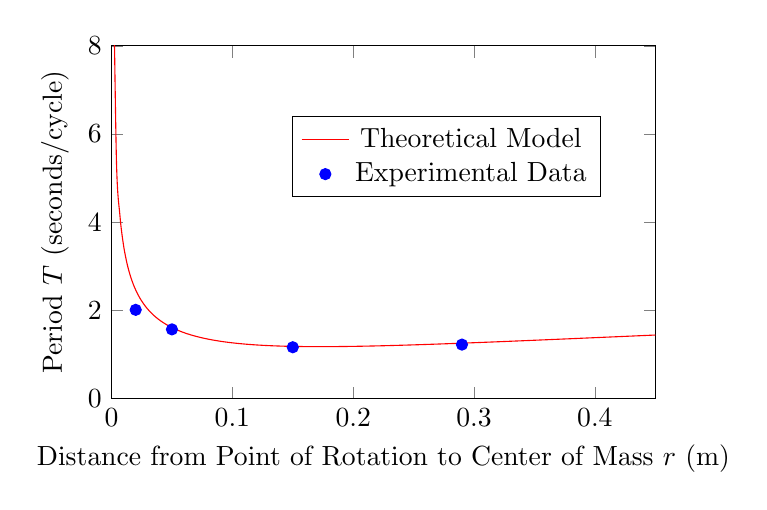
\begin{tikzpicture}[
    declare function={
        T(\r) = 2 * pi * sqrt(2.61530744747 * 10^(-3) / (8.8 * 10^(-2) * \r * 9.8) + \r/9.8);
    },
]
    \begin{axis}[
        xlabel={Distance from Point of Rotation to Center of Mass $r$ (m)},
        ylabel={Period $T$ (seconds/cycle)},
        xtick distance=0.1,
        ytick distance=2,
        domain=0.001:3,
        xmin=0, xmax=0.45,
        ymin=0, ymax=8,
        samples=1000,
        smooth,
        height=.5\textwidth,
        width=.7\textwidth,
        legend entries={Theoretical Model, Experimental Data},
        legend style={at={(0.9, .8)}},
    ]
        \addplot [red]    {T(\x)};
        \addplot[color=blue,mark=*, only marks] coordinates {
            (0.02,2.013)
            (0.05,1.57)
            (0.15,1.165)
            (0.29,1.225)
        };
    \end{axis}
    \end{tikzpicture}
    \caption{Period vs. Distance from Point of Rotation to Center of Mass}
    \label{fig:TvsR}
    \end{figure}
    To find the minimum period, we take the derivative of $T(r)$ and set it equal to zero. This point is at $r\approx 0.1724$, where there is a minimum period of $\approx 1.1785$.
\end{enumerate}
\subsection{Conclusion}
\begin{table}[H]
    \centering
    \begin{tabular}{|c|c|c|c|c|}
        \hline
        $L$ (m) & $r$ (m) & Experimental $T$ (s/cycle) & Theoretical $T$ (s/cycle) & Error $\delta$ (\%) \\
        \hline
        0.32 & 0.02 & 2.013 & 2.463 & 18.27 \\
        0.35 & 0.05 & 1.570 & 1.611 & 2.55 \\
        0.45 & 0.15 & 1.165 & 1.184 & 1.60 \\
        0.59 & 0.29 & 1.225 & 1.257 & 3.20 \\
        \hline
    \end{tabular}
    \caption{Percent Error of Observed Period from Theoretical Period}
    \label{tab:percentError2}
\end{table}
Aside from $r=0.02$, an outlier in the data, the percent error of the observed period from the theoretical period is less than 4\%. \\
\\
From \autoref{tab:solidPendulumData}, we can see that our prediction was partially correct. The pendulum did not oscillate when the point of rotation is at the center of the ruler, $L=0.30 \text{ m}$. This can be seen in \autoref{fig:TvsR} as well, with the vertical asymptote at $r=0$. As the distance from the center of mass increases, the period decreases. However, $T$ at $L=0.59 \text{ m}$ is greater than $T$ at $L=0.45 \text{ m}$. This is potentially due to the change in moment of inertia of the ruler with holes. This behavior can also be seen in \autoref{fig:TvsR}. At $r\approx 0.1724$, the period begins to increase. 
\end{document}
